\section{Background}
\label{sec:background}
The work in this paper falls within the field of natural language grounding.
The grounding problem consists of correctly determining how phrases relate to the real world (e.g. that the phrase ``go to the cube'' means approaching a physical cube).\\
\indent Before proceeding further, one must define the domains over which the grounding problem may be solved.
In the general formulation of the grounding problem, 3 variable domains must be considered: $\Gamma = \{\text{symbolic actions and objects\}}$, which represents what phrases may be grounded to, $\Lambda = \{\text{English phrases}\}$, which represents what phrases natural language sentences may be composed of, and $\Upsilon = \Gamma \times \{\text{object attributes}\} $, which represents a model of the world in which phrases may be grounded.\\
\indent Using these domains, it is possible to formulate the general grounding problem as a probability maximization problem, shown in Equation~\ref{eq:max_ground_prob},
\begin{equation}
\boldsymbol{\gamma}^* = \argmax_{\boldsymbol{\gamma} \epsilon \Gamma^{|\boldsymbol{\lambda}|}} p(\boldsymbol{\gamma}|\boldsymbol{\lambda},\Upsilon),
\label{eq:max_ground_prob}
\end{equation}

\noindent for $\boldsymbol{\gamma}$ defined as a vector of groundings $\gamma \in \Gamma$, $\boldsymbol{\lambda}$ as a vector of phrases $\lambda \in \Lambda$ and world model $\Upsilon$. 
This formulation states that the optimal grounding $\boldsymbol{\gamma}^*$ is the vector of groundings that maximizes the likelihood of that vector of groundings, given language $\boldsymbol{\lambda}$ and a model of the world $\Upsilon$.\\
\indent While the general formulation allows any possible grounding, phrase, or world model, the domains of $\Gamma$, $\Lambda$, and $\Upsilon$ are shrunk in existing solutions to the grounding problem.
For example, rather than allowing $\Lambda$ to include all words, many systems only consider words that have appeared in training examples.\\
\indent Specifically, consider the Distributed Correspondence Graph (DCG), which makes 5 changes to the general grounding problem formulation.
First, DCG discards the notion of grounding to specific actions or objects by instead only grounding to constraints relative to known objects (e.g. the area near a cube) and then passing the constraints to a motion planner.
Second, DCG only allows phrases composed entirely of words that have already been encountered in training.
Third, DCG only considers perceived objects rather than a full model of the world including unobserved objects.
Fourth, ternary correspondence variables $\phi_{ij}$ are introduced to represent whether the $i^\text{th}$ phrase $\lambda_i$ from the overall command $\boldsymbol{\lambda}$ corresponds to a grounding $\gamma_{ij}$.
For a given phrase $\lambda_i$, $\phi_{ij}$ is set to Active if $\lambda_i$ corresponds to constraint $\gamma_{ij}$, Inverted if $\lambda_i$ corresponds to the opposite of $\gamma_{ij}$, or Inactive if $\lambda_i$ has no bearing on $\gamma_{ij}$.
Fifth, for the sake of computational efficiency, the overall inference is factored using conditional independence according to the structure of the parse tree of $\boldsymbol{\lambda}$.
These changes are formally shown in Equation~\ref{eq:dcg_factored1},
\begin{equation}
\label{eq:dcg_factored1}
\begin{split}
\boldsymbol{\phi}^* = \argmax_{\boldsymbol{\phi} \epsilon \Phi^{|\boldsymbol{\lambda}|}} \prod_{ij} p(\phi_{ij}|\gamma_{ij},\lambda_i,\Gamma_{c_{ij}} , \Upsilon),
\end{split}
\end{equation}
where $\Gamma_{c_{ij}}$ is the set of child groundings of $\gamma_{ij}$.
Finally, the domains are redefined for $\gamma \in C=\{\text{Constraints}\}$, $\lambda \in \Lambda_{KN}=\{\text{phrases with known nouns}\}$, and $\Upsilon \in \{\text{object attributes}\} \times \Gamma_{KP}$ for $\Gamma_{KP} = \{\text{known perceived symbolic objects}\}$.\\
\indent As stated previously, DCG assumes conditional independence among groundings, given $\Gamma_{c_{ij}}$.
Child groundings $\Gamma_{c_i}$ may be formally defined as the set of groundings for the leftmost descendants of the immediate children (barring itself) of the parent of phrase $i$ in the parse tree of the natural language command.
This is best illustrated by way of example in Figure~\ref{fig:parse_tree}, showing the parse tree of a simple command, and Figure~\ref{fig:dcg_plates}, showing the corresponding DCG graphical model. 

\begin{figure}
\centering
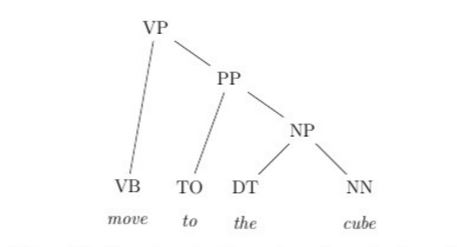
\includegraphics[width=7cm,height=3cm]{parse_tree}
\label{fig:parse_tree}
\caption{Parse tree for the command ``move to the cube''}
\end{figure}

\begin{figure}
\centering
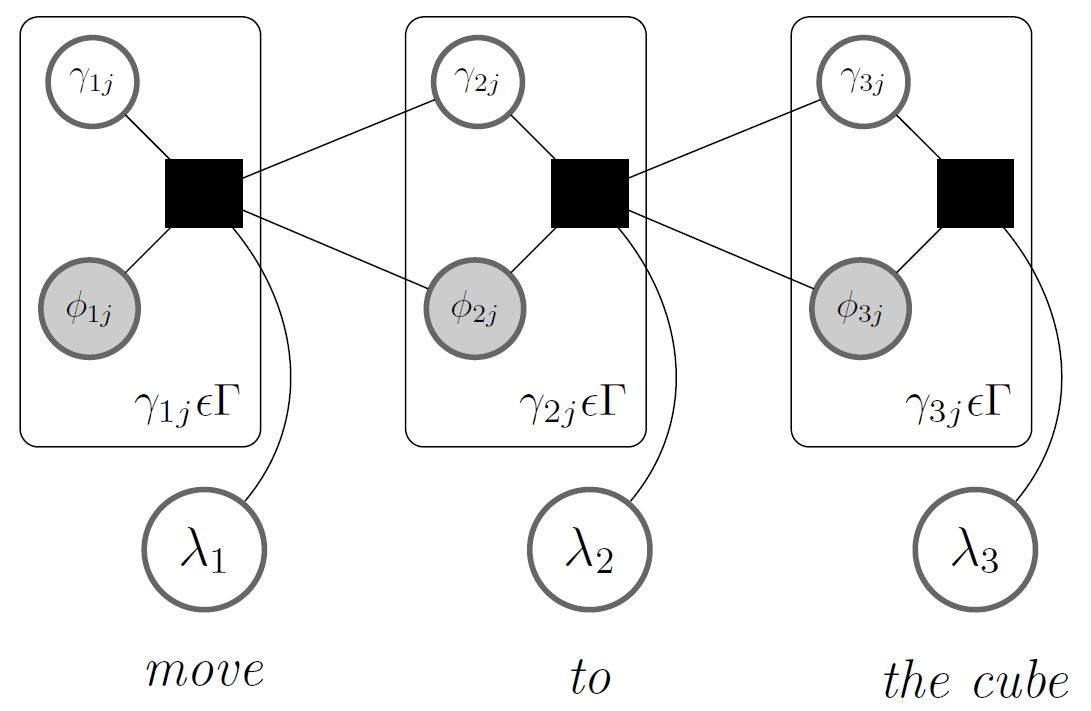
\includegraphics[width=7cm,height=3cm]{dcg_plates}
\label{fig:dcg_plates}
\caption{DCG graphical model for the parse tree in Figure~\ref{fig:parse_tree}}
\end{figure}

In this example, the child grounding of the phrase ``move'' is the grounding for the phrase ``to.''
Similarly, the child grounding of the phrase ``to'' is the grounding for the phrase ``the cube'' (determiners such as ``the'' may be collapsed into their nouns).
Thus, in this example, each grounding has exactly one child grounding, yielding the inter-plate structure in Figure~\ref{fig:dcg_plates}.
Examining the parse tree also reveals why the factorization in Equation~\ref{eq:dcg_factored1} is reasonable: the meaning ``move'' should be conditionally independent of the noun ``cube'' given the prepositional phrase.
After all, the correct grounding of the word ``move'' is an action that does not depend on whether the target is a cube or a sphere, but it does depend on the position of the cube.\\
\indent Finally, one must consider the factor function $\Psi$ within each plate that determines the most likely configuration of each $\phi_{ij}$ given $\lambda_i$, $\gamma_{ij}$, and $\Gamma_{c_{ij}}$.
In order to expose the use of $\Psi$, one may rewrite Equation~\ref{eq:dcg_factored1} as Equation~\ref{eq:llm1}, \\
\begin{equation}
\boldsymbol{\phi}^* = \argmax_{\boldsymbol{\phi} \epsilon \Phi^{|\boldsymbol{\lambda}|}} \frac{1}{Z} \prod_{ij} \Psi(\phi_i,\gamma_{ij},\lambda_i,\Gamma_{c_{ij}},\Upsilon),
\label{eq:llm1}
\end{equation}
where $\Psi$ is set as a log-linear model (LLM) composed of a weighted combination of hand-coded binary function, as shown in Equation~\ref{eq:llm2}:
\begin{equation}
\Psi(\phi_{ij},\gamma_{ij},\lambda_i,\Gamma_{c_{ij}},\Upsilon) = \exp \Big( \sum_{f \epsilon F} \mu_f f(\phi_{ij},\gamma_{ij},\lambda_i,\Gamma_{c_{ij}},\Upsilon) \Big)
\label{eq:llm2}.
\end{equation}
\indent Each binary function $f$ belongs to a set of hand-coded binary features that evaluate specific traits about a grounding (e.g. whether the word ``cube'' appears in $\boldsymbol{lambda}$).
The weights $\mu_f$ used to combine these features are learned in a training procedure based on the Limited-memory Broyden-Feltcher-Goldfarb-Shanno algorithm to generate a more nuanced function that evaluates how likely a phrase is to correspond to a grounding.